\documentclass[14pt,a4paper,oneside]{article}

\usepackage[utf8]{inputenc}   


\usepackage{amsmath,amsthm,amssymb,appendix,bm,mathrsfs,ctex,geometry,tcolorbox,fancyhdr,tikz,esint,appendix}


%% GB/T 7714 宏包 ---- 引文格式
\usepackage[sort&compress]{gbt7714}
\bibliographystyle{gbt7714-numerical}



\numberwithin{equation}{subsection}             %%%%%% 公式编号




\geometry{left=1.7cm, right=1.7cm, top=2.54cm, bottom=2.54cm}    %%%%% 页面尺寸
\linespread{1.5}                             %%%%% 行距1.5倍
\pagestyle{fancy}



%%    设置页眉页脚
\fancyhf{}
\renewcommand{\headrulewidth}{0.15mm}
\fancyhead[C]{文献阅读报告}                   %%%%%% 页眉
\fancyfoot[C]{\thepage}                      %%%%%% 页脚 页码
\setlength{\headheight}{15pt}


%%   设置各种链接颜色为黑色
\usepackage[colorlinks,
            linkcolor=black,
            anchorcolor=black,
            citecolor=black,
            urlcolor=black
            ]{hyperref}



%%   例子编号
\newcounter{example}
\counterwithin{example}{subsection}
\newcommand{\examplename}{Example}
\newcommand{\exampleTitle}[1]{%
\textbf{\refstepcounter{example}\examplename\theexample:#1}\par}


%%  插入图片配置
\usepackage{graphicx,subfigure}
\usepackage[]{caption2} %新增调用的宏包
\numberwithin{figure}{subsection}               %%%%%% 图片编号

\graphicspath{ {./Figure/} }            %%%%% 设置图片文件所在目录
\DeclareGraphicsExtensions{.pdf,.svg,.jpeg,.png,.jpg}     %%%%% 支持图片格式


%%    支持tikz作图
\usepackage{tikz}
\usetikzlibrary{backgrounds,arrows}


\usepackage{pgfplots}
\pgfplotsset{compat=1.15}
\usepackage{mathrsfs}


\title{\textbf{文献阅读报告 9\\High-energy pulse self-compression and ultraviolet generation through soliton dynamics in hollow capillary fibres}}                           %%%%% 标题
\author{骆禹天}                                           %%%%% 作者
\date{2024/**/**}                                        %%%%%% 日期

%%   定义一些数学格式
\newtheorem{theorem}{定理}[subsection]
\newtheorem{definition}[theorem]{定义}
\newtheorem{lemma}[theorem]{引理}
\newtheorem{corollary}[theorem]{推论}
\newtheorem{example}[theorem]{例}
\newtheorem{proposition}[theorem]{命题}
\renewcommand{\abstractname}{\Large\textbf{摘要}}




%------------------------- 开始文档  -------------------------%



\begin{document}

\pagenumbering{Roman}         %%%%% 目录前页码统计按罗马数字

\maketitle

\setcounter{page}{1}          %%%%% 标题开始统计页数

%------------------------- 目录  ------------------------------%

\tableofcontents              %%%%% 插入目录

\newpage
\setcounter{page}{1}          %%%%% 目录后重新统计页数


\pagenumbering{arabic}        %%%%% 目录后统计页码为阿拉伯数字



%%%%%%%%%%%%%%%%%%%% 开始第一节  %%%%%%%%%%%%%%%%%%%%%


\section{Introduction}

空心毛细管光纤 (HCF) 由玻璃纤维中的简单圆形孔组成. 应用: 频率转换和放大

· 四波混频\cite{durfeeUltrabroadbandPhasematchedOptical1997, kidaOpticalParametricAmplification2014};

· 真空紫外 (VUV) 生成\cite{misogutiGenerationBroadbandVUV2001};

· 时空自压缩\cite{wagnerSelfCompressionUltrashortPulses2004, andersonHighenergyLaserpulseSelfcompression2014, gaoIonizationassistedSpatiotemporalLocalization2018};

· 高次谐波生成\cite{durfeeiiiPhaseMatchingHighorder1999, popmintchevBrightCoherentUltrahigh2012};

· 液体中的非线性光学\cite{chemnitzHybridSolitonDynamics2017};

· 在超快光学中, 主要应用是基于非线性光谱展宽的脉冲压缩\cite{nisoliGenerationHighEnergy1996, nisoliTerawattscaleSub10fsLaser1998};

值得注意, 在此之前有一类非常重要的非线性效应未在充气 HCF 中得到证实: 光学孤子以及与之相关的丰富动力学. 

光学孤子的形成: 通过正的非线性折射率与负 (反常) 色散间的平衡. 它们是非线性光学 (尤其是光纤) 中许多重要现象的基础例如:

· 极端脉冲自压缩\cite{mollenauerExtremePicosecondPulse1983, imHighpowerSolitoninducedSupercontinuum2010, jolyBrightSpatiallyCoherent2011, makTwoTechniquesTemporal2013, balciunasStrongfieldDriverSinglecycle2015}、

· 白光超连续谱的形成\cite{dudleySupercontinuumGenerationPhotonic2006} 

· 通过谐振色散波 (RDW) 发射有效生成频率可调脉冲\cite{imHighpowerSolitoninducedSupercontinuum2010, jolyBrightSpatiallyCoherent2011, waiNonlinearPulsePropagation1986, makTunableVacuumUVVisible2013, belliVacuumultravioletInfraredSupercontinuum2015, ermolovSupercontinuumGenerationVacuum2015, brombergerAngleresolvedPhotoemissionSpectroscopy2015, kottigGenerationMicrojoulePulses2017}. 

人们认为, HCF 在可见光和近红外 (NIR) 区域不可能实现这些效果因为这些光谱范围的色散较弱. 

充气中空光纤 HCF $\mathrm{HE_{nm}}$ 模式的群速度色散 (GVD) 由下式给出
\begin{equation}
    \beta_2(\lambda)\approx\frac{\lambda^3}{4\pi c^2}\left(\rho_\mathrm{r}\frac{\partial^2\chi_\mathrm{e}}{\partial\lambda^2}-\frac{u_{nm}^2}{2\pi^2a^2}\right)
    \label{eq:1.0.1}
\end{equation}
其中 n 和 m 是模式指数, $u_{nm}$ 是贝塞尔函数 $J_{n-1}$ 的第 m 个零, a 是 HCF 纤芯半径, $\lambda$ 是波长, $\rho_r$ 是相对于某个标准的气体密度条件下, $\chi_e(\lambda)$ 是这些标准条件下气体的线性电化率. 

由于方程\ref{eq:1.0.1} 中的第一项在几乎所有气体的光学波长下均为正值, 因此只能使用第二项 (描述波导的色散) 获得负 GVD. 重要的是, 对较大纤芯尺寸, HCF 能产生的贡献较弱. 

而空心光子晶体光纤 (HC-PCF) 尽管其纤芯半径较小 (通常约为 15 $\mathrm{\mu m}$) , 但可提供低损耗引导, 从而产生足够的反常波导色散, 以便在低脉冲能量下观察到孤子效应. 相比之下, 如此小的纤芯, 传统 HCF 的损耗高得惊人\cite{marcatiliHollowMetallicDielectric1964}.  1/e 倍的功率损耗长度由下式给出
\begin{equation}
    L_\mathrm{loss}\approx\frac{4\pi^2a^3}{3u_{nm}^2\lambda^2}
    \label{eq:1.0.2}
\end{equation}
在 800 nm 波长、半径 15 $\mathrm{\mu m}$ 的 HCF 中, $\mathrm{HE_{11}}$ 模式的功率损耗长度仅为 1 cm. 

使用具有更大纤芯半径 ($\sim$ 75-500 $\mathrm{\mu m}$) 的 HCF 可以显着降低损耗 ($L_{\mathrm{loss}} \propto  a^3$), 且还允许比 HC-PCF 更高的脉冲能量和峰值功率, 但会极大地降低了波导色散, 因此气体非线性占主导地位. 在传统的HCF脉冲压缩中, 中空光纤中的传播仅用于通过非线性自相位调制 (SPM) 和自陡峭来增加脉冲带宽, 并且HCF中的色散被忽略. 相反, 光纤后的啁啾镜提供暂时压缩脉冲所需的负二次相位 (称为后压缩) . 如图 \ref{p1.0.1} a, 通过这种方式, 可以在高达几毫焦耳的高脉冲能量下实现对几个甚至单周期脉冲的压缩. 

关于如何在 HCF 中获得孤子效应 (需要非线性和色散在光纤内同时作用) 的理论建议包括使用金属涂层 HCF 来减少损耗、以高阶模式泵浦以增加方程\ref{eq:1.0.1}中的$u_{mn}$\cite{lopez-zubietaTheoreticalAnalysisSinglecycle2018, lopez-zubietaSpatiotemporaldressedOpticalSolitons2018}, 或转向更长的波长\cite{zhaoSelfcompression8mmPulses2017, voroninSubcycleSolitonicBreathers2014}. 然而目前为止, 仅报道了自压缩的数值结果, 而各种孤子效应仍未被探索, 且迄今为止尚未进行任何实验. 

\begin{figure}[h]
    \centering
    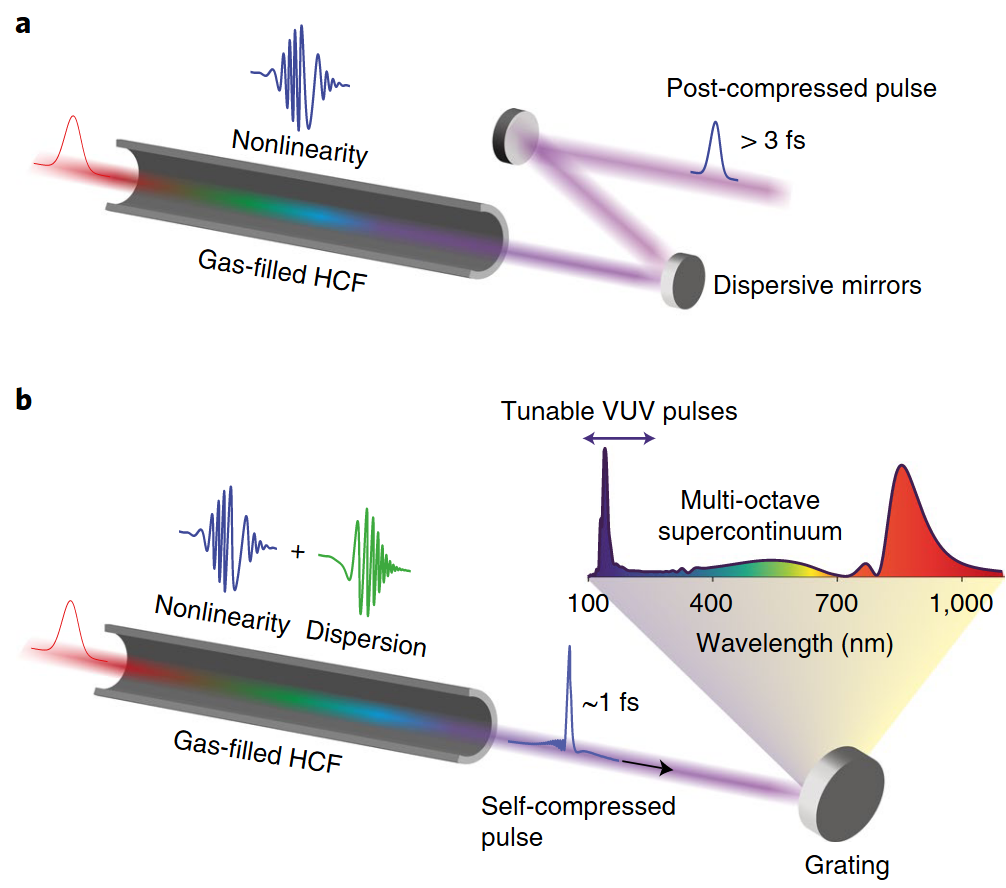
\includegraphics[width=0.4\textwidth]{p1.png}
    \caption{HCF 中后压缩和孤子动力学的比较.  a, 传统后压缩, 主要基于自相位调制和自陡峭的非线性光谱展宽, 反常色散由啁啾镜提供.  b, 孤子动力学, 结合了非线性和色散导致极端的自压缩、紫外生成和多倍频程超连续谱. }\label{p1.0.1}
\end{figure}

\section{Results}

\subsection{Scaling rules for soliton dynamics in HCF}

超短脉冲传播的特性取决于完全依赖于波长的色散情形以及非线性与色散间平衡. 这种平衡的特征是泵孤子阶数
\begin{equation}
    N = \sqrt{L_{\mathrm{d}}/L_\mathrm{{nl}}},  
    \label{eq:2.1.1}
\end{equation}
其中色散长度 $L_{\mathrm{d}}$ 和非线性长度 $L_\mathrm{{nl}}$ 分别描述了 GVD 和 SPM 的特征长度尺度. 

在 HCF 中, 色散情形的合理参数化是泵浦波长 $\lambda_0$ 相对于零色散波长 $\lambda _{\mathrm{zd}}$ 的相对位置 (通过 $\beta_2(\lambda _{\mathrm{zd}}) = 0$ 定义) . 这决定了 RDW 生成的相位匹配位置, 因此, 在 $\lambda _0$ 固定的通常情况下, 改变 $\lambda _{\mathrm{zd}}$ (通过气压) 可以调整 RDW 发射波长. 这还决定了可实现高质量自压缩的程度. 为了获得最强的不受扰动压缩, 需要一个广泛的反常色散区域, 需要将 $\lambda _{\mathrm{zd}}$ 调整得远离 $\lambda _0$. 

图 \ref{p2.1.1} 显示了 800 nm 处 10 fs 脉冲在不同芯尺寸的充氦中空光纤中传播的数值模型. 

· 不同纤芯尺寸, 作者调整气压使 $\lambda _{\mathrm{zd}} = 380 nm$ (与稍后自压缩实验匹配) , 

· 调整能量将孤子阶数维持在 N = 2.6

· 因此, 即使能量增加近三个数量级 (0.006 mJ 至 3 mJ) , 得到几乎相同的时间和光谱动力学. 

· 微小差异由每种情况不同传播损耗造成. 

· 这种缩放是气体中非线性光学一般缩放的一种表现, 当应用于中空纤维时相当于将核心半径缩放一个因子 $\eta$, 如果将气体压力也按 $1/\eta^2$ 缩放, 并将光纤长度和峰值功率按 $\eta^2$ 缩放, 则会出现完全相同的动力学 (不包括损耗) . 

\begin{figure}[h]
    \centering
    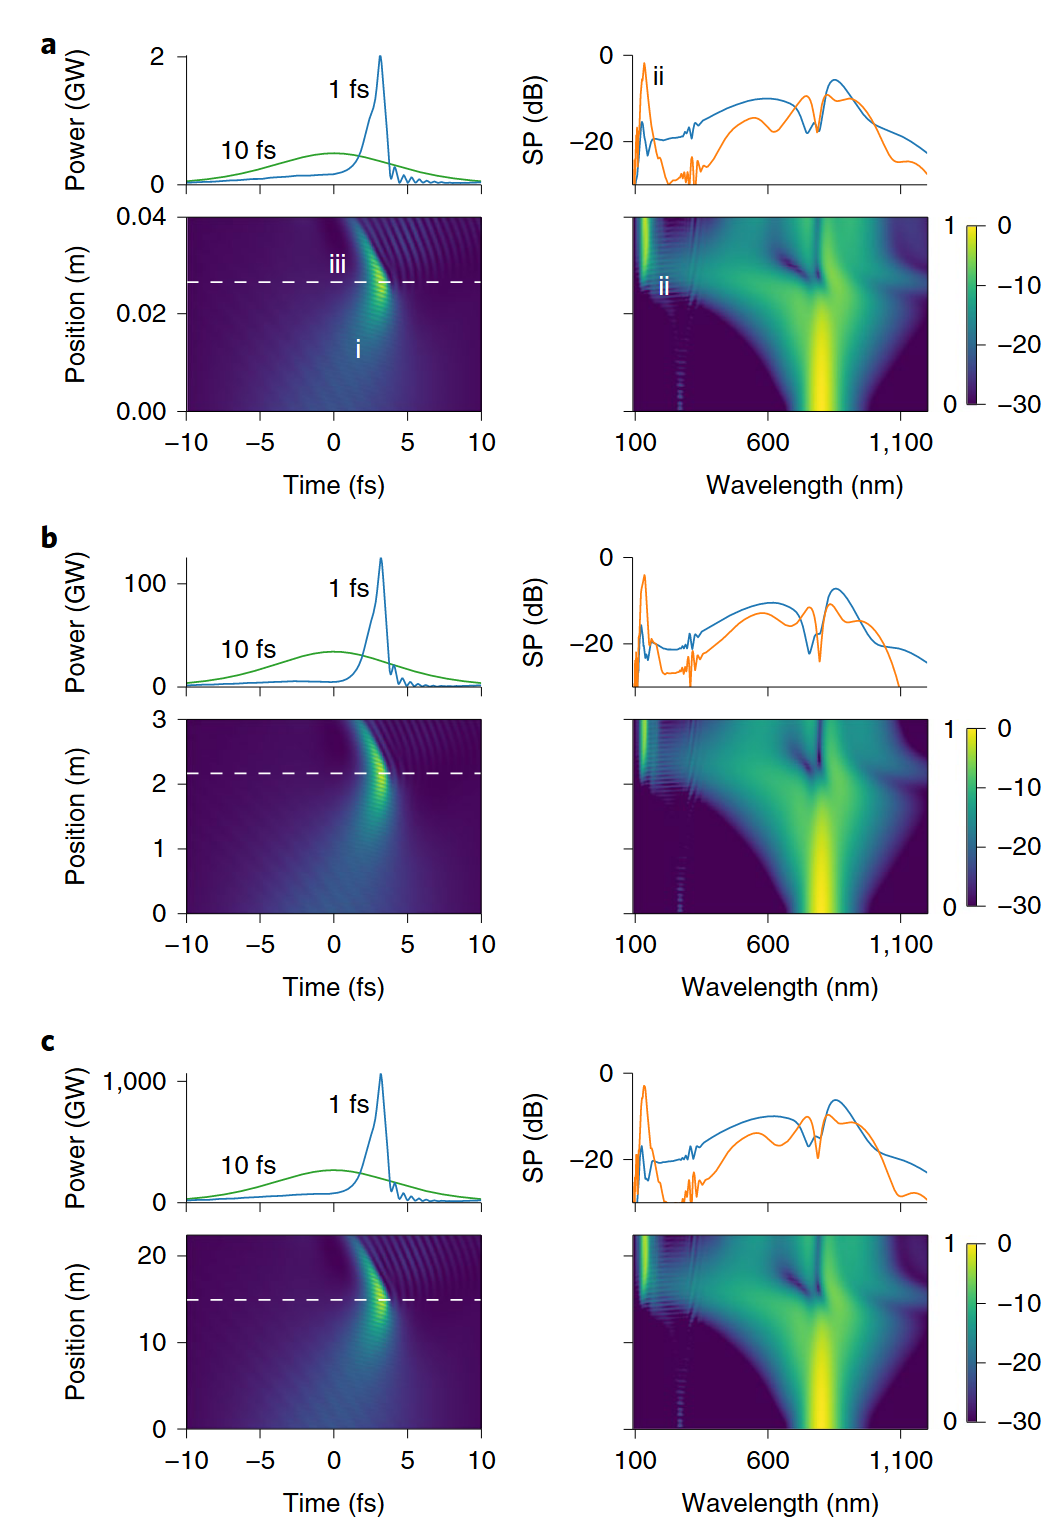
\includegraphics[width=0.5\textwidth]{p2.png}
    \caption{HC-PCF中孤子动力学数值模拟, 中空光纤中充He, $\lambda _{\mathrm{zd}}$ = 380 nm, 10 fs、N = 2.6 孤子, 中心波长 $\lambda _0 = 800\; nm$ : a. 小纤芯动力学示例, 类似于 HC-PCF (但忽略共振) , 无损耗: a = 15 $\mathrm{\mu m}$, 27.8 bar He, 能量 0.006 mJ; b. HCF, a = 125 $\mathrm{\mu m}$, 400 mbar He, 能量 0.4 mJ; c. HCF, a = 350 $\mathrm{\mu m}$, 51 mbar He, 能量 3 mJ}\label{p2.1.1}
\end{figure}

· 能量扩展:

图 \ref{p2.1.1} a 中, 低能量结果对应没有任何损耗的理想小纤芯反谐振引导 HC-PCF. 真正的 HC-PCF 中, 其制导机制固有的包层共振会产生多个大损耗和色散的共振带, 特别是在光谱的 VUV 部分. 然而, 类似于图 \ref{p2.1.1} a 中动力学先前已被证明并用于角分辨光电子能谱和时间分辨光电子成像光谱. 图 2b、c 显示了简单、非微结构的 HCF 结果.  HCF 中较大的纤芯尺寸可实现显着的能量扩展. 

· 自压缩:

(标记 i), 因为泵浦脉冲参数对应于在负色散区域中传播的高阶孤子 (N > 1). 因此, 最初 SPM 占主导, 脉冲频谱展宽; 这增强了负 GVD 效果, 从而补偿非线性相位并导致脉冲和随后的孤子裂变动力学的时间压缩. 可看到这种自压缩产生 1 fs 脉冲. 对于小纤芯情况, 此 1 fs 脉冲达到 2 GW 的峰值功率, 而在最大纤芯中, 可缩放至 1.2 TW. 

· 超连续生成:

而在频域中, 自压缩对应于从 100 nm 开始跨越四个倍频程的超连续谱 (蓝色谱线图) . 随后的光谱动态显示所有纤芯尺寸的 130 nm 左右的有效 RDW 发射 (标记 ii), 图 \ref{p2.1.1} a-c 的 VUV 能量分别为 0.6、25 和 300 $\mathrm{\mu J}$. 而后作者通过光谱过滤提取 VUV 脉冲. 它们的最大峰值功率分别为 0.2、6 和 80 GW, 脉冲持续时间为 1.8 fs, 带宽限制为 0.8 fs. 

· 电离与等离子体效应:

由于图 \ref{p2.1.1} 中的高强度 (在所有情况下高达$ 8 \times 1014\; \mathrm{W\;cm^{-2}}$) ,  0.3\% 的气体被电离 (导致 40\% 的能量损失) , 且产生等离子体效应. 特别是, 孤子自频蓝移以及相应的孤子加速 (标记 iii 的时域图中孤子的弯曲轨迹来识别) 是明显的, 并且这些都改变并增强了 VUV RDW 发射的强度. 自压缩和 RDW 发射不需要这些效应, 在模拟中即使关闭电离和等离子体效应, 这两种效应仍然会发生, 或者对于需要较低脉冲强度的其他参数组 (较高的压力和更长的 $\lambda _{\mathrm{zd} }$) . 

图 \ref{p2.1.1} 还是 HCF 中孤子动力学的具体示例. 一般来说, 会希望能改变泵浦脉冲持续时间、零色散波长 $\lambda _{\mathrm{zd} }$ (调节 RDW 发射波长) 和纤芯尺寸 (以控制能量和功率水平) . 为了确保孤子动力学不被 HCF 损失排除, 需保持 $L_{\mathrm{fiss}} < L_{\mathrm{loss}}$, 其中$ L_{\mathrm{fiss}} \approx L_\mathrm{d}/N$ 是孤子裂变长度, 近似于孤子自压缩和后续脉冲分裂所需的长度尺度. 可以证明 HCF 中该长度为
\begin{equation}
    L_\mathrm{fiss}\approx\frac{a^2\tau_\mathrm{fw}^2}{\text{з}N\mid\delta(\lambda_0,\lambda_\mathrm{zd})|}\propto\frac{a^2\tau_\mathrm{fw}}{\sqrt{I_0}}
    \label{eq:2.1.2}
\end{equation}
其中 $\tau_{\mathrm{fw}}$ 是脉冲时域半高全宽, $I_0$ 是峰值强度, $\delta(\lambda , \lambda _{\mathrm{zd}})$ 是描述填充气体色散的函数. 

图 \ref{p2.1.1} 显示了中心波长 $\lambda _0 = 800 \mathrm{nm}$ 下的缩放规则, 作为两个 $\lambda _{\mathrm{zd} }$ 示例值的纤芯半径和泵浦脉冲持续时间的函数. 通过查找最大 N 或 $I_0$ 来获得每个脉冲持续时间的最小 $L_{\mathrm{fiss}}$, 该最大 N 或 $I_0$ 由多个因素决定:

· 首先, 为了获得相干的孤子自压缩而不是非相干的调制不稳定的动力学, 必须确保 N < 15\cite{dudleySupercontinuumGenerationPhotonic2006}. 

· 其次, N 随着泵浦脉冲的峰值功率和强度而增加, 但它们分别受到自聚焦\cite{fibichCriticalPowerSelffocusing2000}和电离的限制. 

\begin{figure}[h]
    \centering
    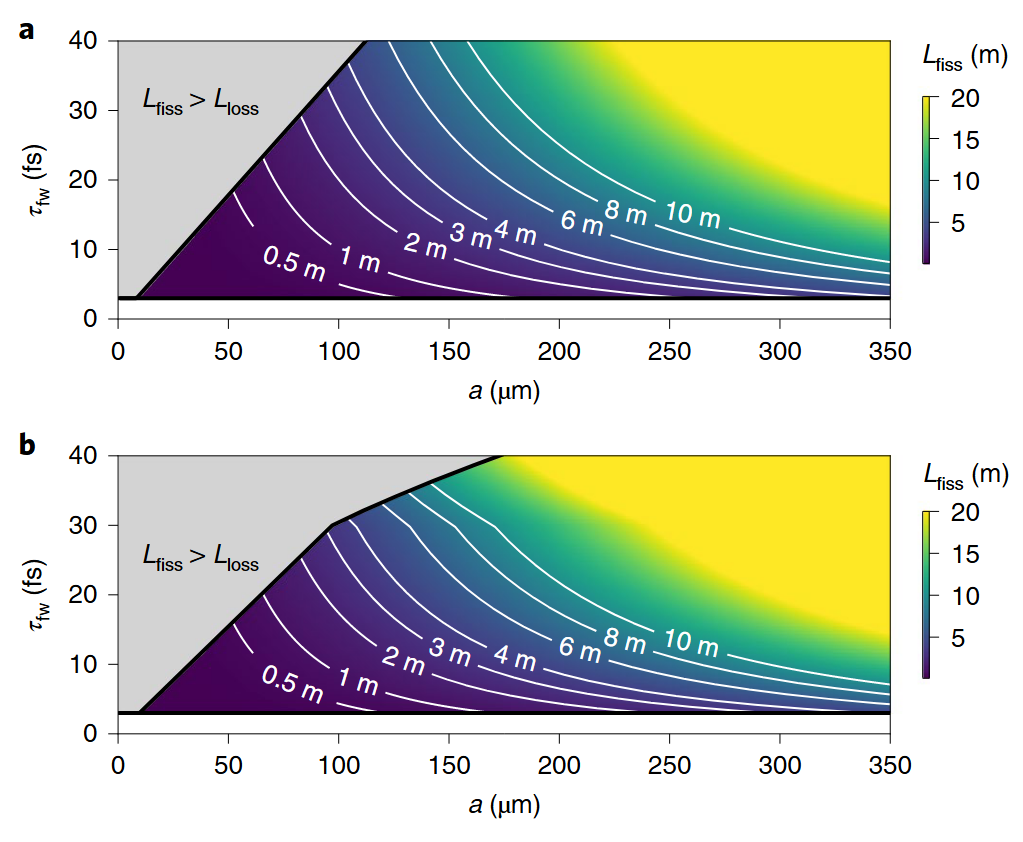
\includegraphics[width=0.5\textwidth]{p3.png}
    \caption{充氦 HCF 中的孤子裂变长度缩放.  a,b, 等值线和色标显示最小孤子裂变长度 $L_{\mathrm{fiss}}$, 使用最大允许 N 根据方程 (3) 计算得出, 作为纤芯半径 a 和脉冲持续时间 $\tau_{\mathrm{fw}}$ 的函数, 其中 $\lambda _0$ = 800 nm 和 $\lambda _{\mathrm{zd} }$ = 380 nm (a) 和 $\lambda _{\mathrm{zd} }$ = 700 nm (b). 在灰色阴影区域, 不可能获得 $L_{\mathrm{fiss}}$ < Lloss. }\label{p2.1.2}
\end{figure}

图\ref{p2.1.2}a、b中的灰色区域显示了由于传播损耗太高且$L_{\mathrm{fiss}} > L_{\mathrm{loss}}$而无法观察孤子动力学的区域. 这种情况发生在纤芯尺寸小和脉冲持续时间较长的情况下. 然而, $L_{\mathrm{fiss}} \propto  a^2$, 而 $L_{\mathrm{loss}} \propto  a^3$ (方程 (\ref{eq:1.0.2}) 和\ref{eq:2.1.1}) , 因此移动到更大纤芯尺寸总是可获得 $L_{\mathrm{fiss}} < L_{\mathrm{loss}}$ (图 \ref{p2.1.2}a、b 的右侧) , 以增加所需的 HCF 长度为代价. 反过来, 这个问题可通过更短的脉冲泵浦来弥补, 如10 fs 或更短的持续时间可使纤芯半径高达 a = 200 $\mathrm{\mu m}$ 的裂变长度保持在 3 m 以下, 对于最小纤芯尺寸, 裂变长度甚至低于半米. 

直到最近, 大多数传统的 HCF 后压缩系统的 HCF 长度仅限于 $\sim$1 m. 这比通常使用的 800 nm 30 fs 泵浦脉冲的裂变长度短得多, 这解释了为什么以前在 HCF 中没有观察到孤子裂变动力学. 

\subsection{High-energy soliton self-compression}

HCF 中自压缩的初步实验:

· Ti:sapphire 系统直接产生脉冲, 持续时间为 26 fs;

· 使用了 3 m 长、纤芯半径 125 $\mathrm{\mu m}$的拉伸 HCF. 

· 最大能量 400 $\mathrm{\mu J}$ 

· 充 1 bar He  ($\lambda _{\mathrm{zd}} = 470 \mathrm{nm}$) , 

· 孤子阶数 N = 6.8, 相应裂变长度为 4.2 m. 

虽 HCF 太短无法达到裂变点, 但图 \ref{p2.2.1} a 显示了当增加泵浦能量 (以及孤子阶数) 时自压缩从 26 fs 到 9 fs 的清晰实验证据. 此外, 作者的数值模型在功率谱 (图 \ref{p2.2.1} b) 和时域脉冲形状的细节 (图 \ref{p2.2.1} a) 都非常接近实验. 

\begin{figure}[h]
    \centering
    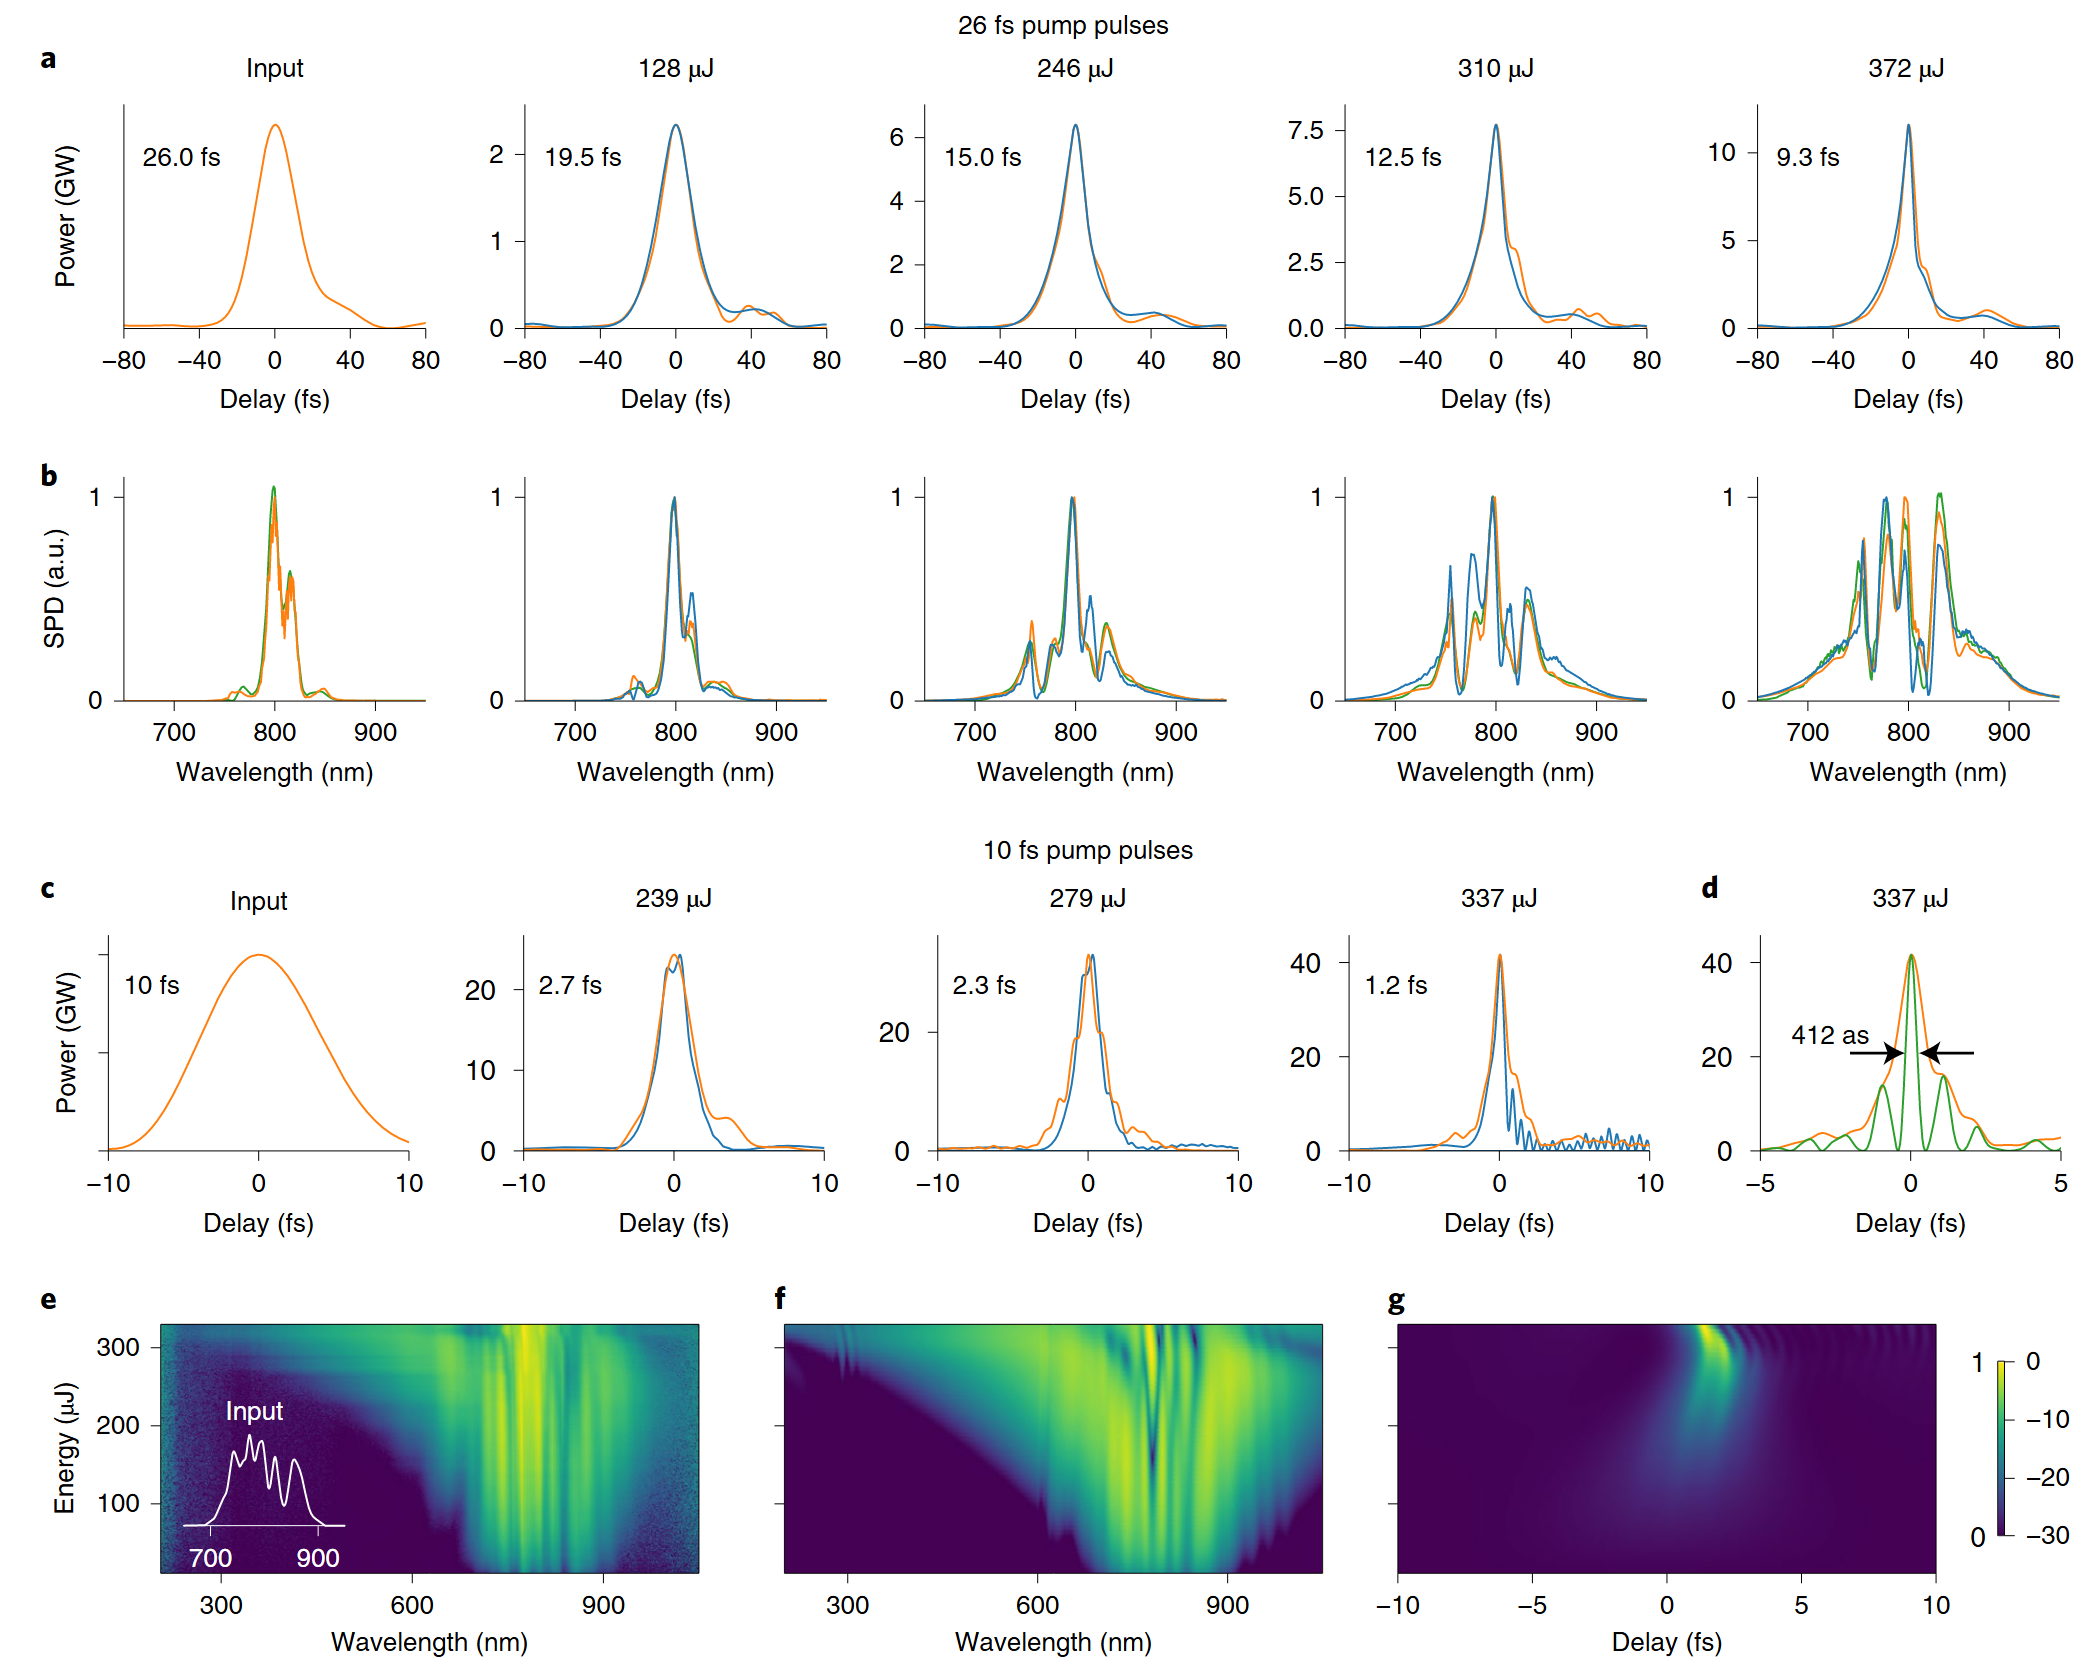
\includegraphics[width=0.9\textwidth]{p4.png}
    \caption{充气 HCF 中的孤子自压缩. a、b: 1 bar He, 26 fs 泵脉冲, a. 用于增加泵浦能量的时间脉冲压缩: 橙色; 通过二次谐波频率分辨光门控 (SHG-FROG) 脉冲检索测量; 蓝色, 数值模型. b. 对应脉冲谱: 橙色, FROG检索到; 蓝色, 数值模型; 绿色, 独立测量.  c-g, 0.4 bar He, 10 fs 泵浦脉冲.  c. 用于增加泵浦能量的时间脉冲压缩: 橙色, 通过 PG-FROG 脉冲检索测量; 蓝色, 数值模型.  d. c 的近距离视图, 但检索到的电场的平方以绿色显示. 请注意正文中描述的 c 和 d 中所示脉冲形状的测量限制.  e. 测量增加泵浦能量的光谱. 插图: 线性尺度上的泵浦光谱.  f. 相应的数值模拟频谱.  g. 相应的数值模拟时间脉冲形状. 所有结果均针对 3 m 长、芯半径为 125 $\mathrm{\mu m}$ 的 HCF. }\label{p2.2.1}
\end{figure}

为观察完整孤子自压缩, 作者从传统 HCF 后压缩设置中产生的 10 fs 泵浦脉冲开始. 如图 \ref{p2.2.1} c-e 所示, 在压力为 0.4 bar ($\lambda _{\mathrm{zd}} = 380 \mathrm{nm}$) 和能量为 239 $\mathrm{\mu J}$ (N = 2) 时获得了从 10 fs 到 2.7 fs 的自压缩, 接近于单周期且只比变换极限稍宽2.5 fs. 随能量增加, 脉冲变短, 279 $\mathrm{\mu J}$ 时压缩至 2.3 fs (变换极限为 2.1 fs) , 最后在 337 $\mathrm{\mu J}$ 时压缩至 1.2 fs, 变换极限为 1.1 fs. 此时, 方场轮廓的全宽度 (如图 4d 所示) 仅为 412, 因为孤子已自压缩为光学阿秒脉冲\cite{hassanOpticalAttosecondPulses2016}. 

说明: 

1. 关于阿秒级脉冲测量技术

脉冲测量基于新型偏振选通频率分辨光选通 (PG-FROG) 技术, 覆盖 200 nm 至 >1,100 nm 波段, 支持 1 fs 子周期脉冲带宽. 然而必须指出该技术有一些严重局限性, 并且子周期脉冲持续时间不能仅根据 PG-FROG 测量可靠地确定. 图 \ref{p2.2.1} 所示的脉冲轮廓是通过测量脉冲通过色散材料 (最显着的是 HCF 系统的出射窗和实验室空气) 传播而被拉伸后获得的, 然后以数值方式将它们反向传播到出口 HCF 的. 一般来说, 这个过程是严格的, 空气、二氧化硅和氟化镁的折射率得到了很好的表征. 对于 2.7 fs 脉冲, 反向传播脉冲持续时间在传播距离和窗口厚度的实验不确定性范围内变化小于 5\%. 然而, 子周期脉冲的极端带宽和延伸至紫外线意味着玻璃厚度仅 10 $\mathrm{\mu m}$ 的差异就足以将 1.2 fs 脉冲拉伸 2.5 倍. 由于 PG-FROG 始终需要透射交互介质, 即使将设备置于真空中也无法避免这个问题. 完全独立的实验证据只有通过更复杂的实验才能提供, 如 attosecond streakin\cite{hassanOpticalAttosecondPulses2016, wirthSynthesizedLightTransients2011}. 

还有两个额外观察结果清楚表明作者实验中产生了光学阿秒脉冲:

(1) 所有实验数据和数值模型间良好的一致性. 

(2) RDW 发射需要压缩到子周期脉冲才能在 VUV 波长范围内发生. 这可以从 RDW 发射的级联四波混合图中理解, 其中 RDW 和泵之间的所有频率需要同时出现. 从补充图 1 中的频谱图中可以清楚地看出这种情况. 对于 VUV 中的 RDW 发射, 同时存在跨越三个倍频程的频率, 这对应于时域中的子周期脉冲. 在 HC-PCF 中也发现了 VUV RDW 发射和子周期脉冲生成之间的相关性. 因此, 作者对 VUV 上 RDW 发射的测量 (见下文) 也支持了 HCF 中存在这种极端脉冲压缩；特别是, 图 \ref{p2.2.1} c 中 1.2 fs 脉冲的参数与图 5a 中所示 130 nm RDW 的参数相同. 

\subsection{Tunable vacuum and deep ultraviolet pulse generation}

在极端压缩点, 孤子由于高阶线性和非线性效应而破裂, 例如自陡峭、激波形成和高阶色散\cite{dudleySupercontinuumGenerationPhotonic2006, beaudUltrashortPulsePropagation1987, kodamaNonlinearPulsePropagation1987, husakouSupercontinuumGenerationHigherorder2001}. 后者引起 RDW 发射, 通常称为光纤-光学切伦科夫辐射或共振辐射 (resonant radiation) \cite{imHighpowerSolitoninducedSupercontinuum2010, jolyBrightSpatiallyCoherent2011, waiNonlinearPulsePropagation1986, makTunableVacuumUVVisible2013, ermolovSupercontinuumGenerationVacuum2015, kodamaNonlinearPulsePropagation1987, husakouSupercontinuumGenerationHigherorder2001, erkintaloCascadedPhaseMatching2012, akhmedievCherenkovRadiationEmitted1995}.  HCF 中 RDW 过程模拟如图 \ref{p2.1.1} 所示, RDW 发射发生在标记 ii. 发射波长取决于色散景观, 因此取决于气体压力和纤芯尺寸 (方程\ref{eq:1.0.1}) .

\begin{figure}[h]
    \centering
    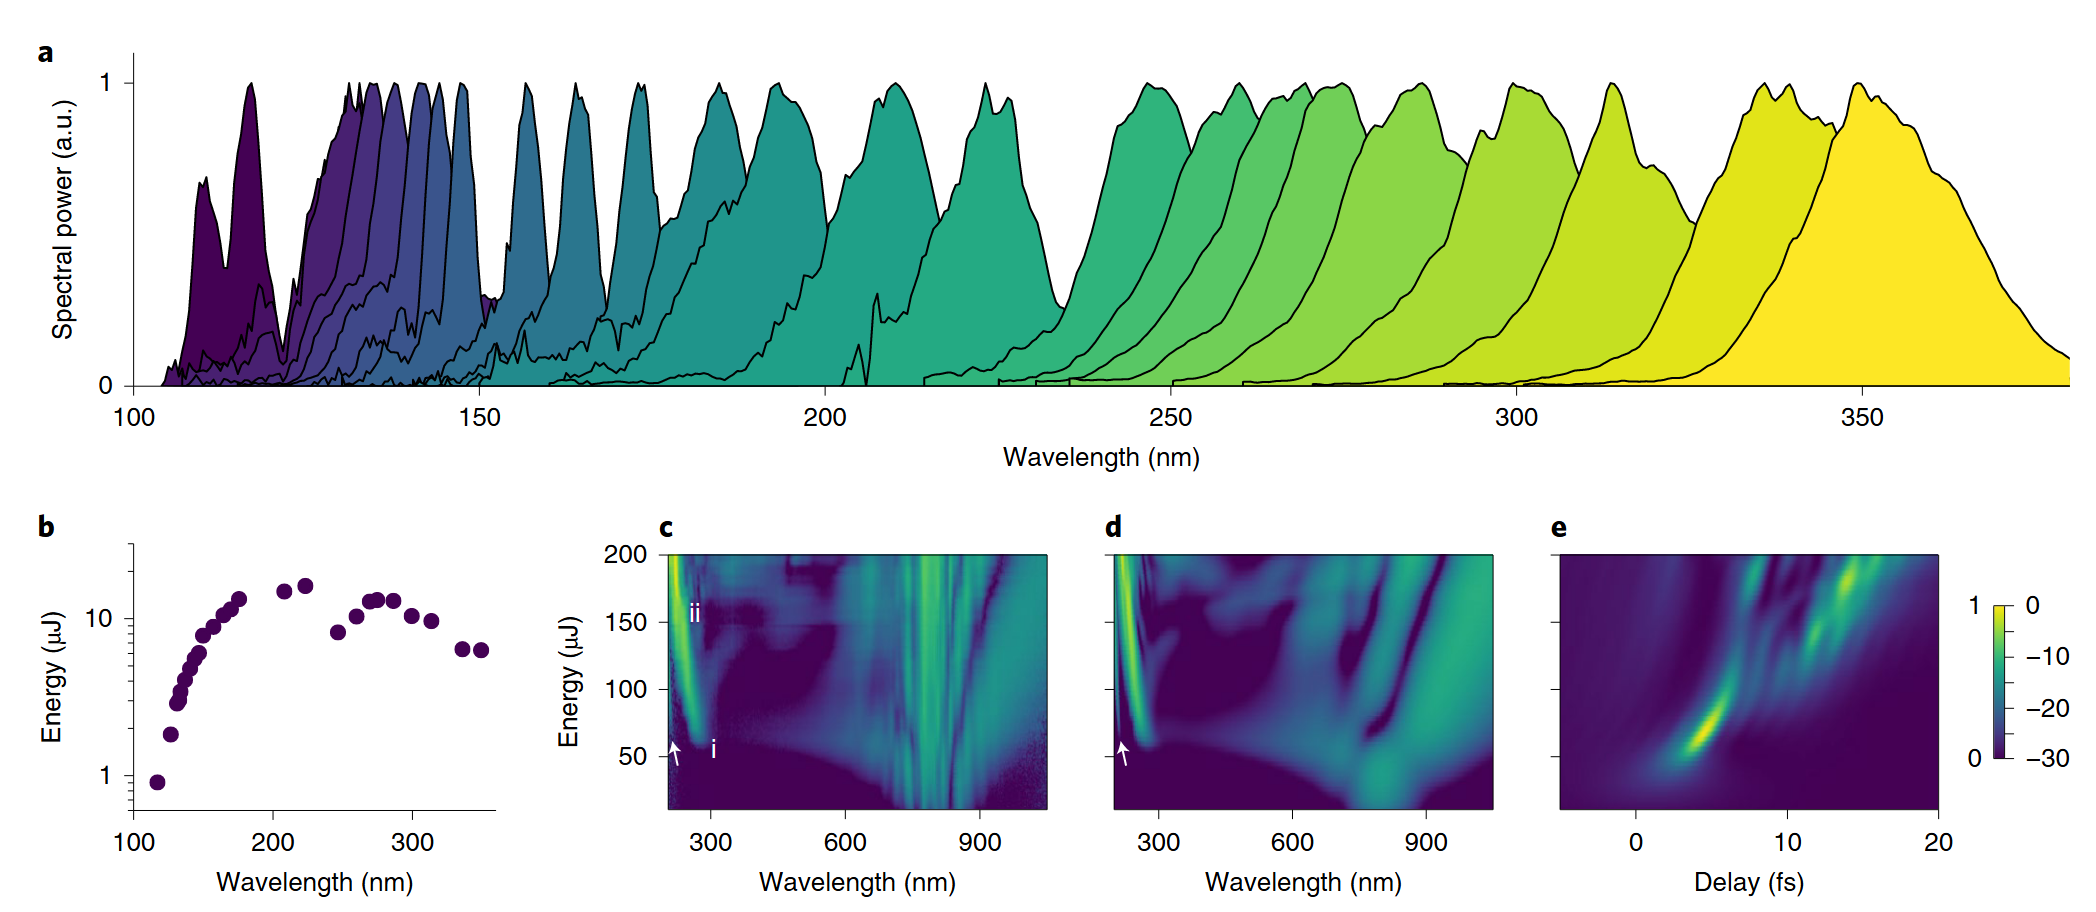
\includegraphics[width=0.9\textwidth]{p5.png}
    \caption{充气 HCF 中可调 rDW 发射.  a 测量的 3 米长 HCF 的 RDW 光谱, 纤芯半径 125 $\mathrm{\mu m}$, He, 10 fs 脉冲泵浦 (泵浦光谱如图 \ref{p2.2.1}e 的插图所示), 压力范围为 230 mbar (最短波长光谱) 至 4 bar (最长波长光谱). 更高压力下还测量到超过 400 nm 的扩展;  b 测得 VUV 至 DUV 脉冲能量;  c 1 bar Ne, 10 fs 泵浦脉冲 HCF 输出处光谱演变作为输入脉冲能量的函数;  d 相应的数值模拟;  e, 相应的时间功率数值模拟.  c, d: 30 dB 对数色标, e: 线性色阶上, c和d中的白色箭头表示$\mathrm{HE_{12}}$模式下的RDW发射. }\label{p2.3.1}
\end{figure}

图 \ref{p2.3.1} a 显示了在 10 fs 脉冲泵浦的 125 $\mathrm{\mu m}$ HCF 中, 通过改变气压将 RDW 发射从 110 nm 以下调整到 350 nm 的实验 (完整参数在补充表 1) . 在更高压力下获得了超过 400 nm 的进一步调谐. 由于纤芯尺寸较大, VUV 中发射的脉冲能量比 HC-PCF 中获得的脉冲高出 1000 倍, 如图 \ref{p2.3.1} b 和补充表 1 和 2 所示. 即使在最短的 RDW 波段 (跨越 107-121 nm, 能量约为1 $\mathrm{\mu J}$)；在 180 nm 附近增加到约 13 $\mathrm{\mu J}$, 在 220 nm 附近增加到 16 $\mathrm{\mu J}$ 左右, 并保持在 10 $\mathrm{\mu J}$ 左右, 直到在 300 nm 处开始减少, 因为在较高压力下所需的泵浦能量较低.  VUV 的估计转换效率范围为 120 nm 左右的 0.5\% 到 170 nm 左右的 5\%, 而在深紫外 (DUV, 200 nm 至 300 nm) 中, 该转换效率会增加到 15\% 以上 (补充表 1) . 整个系统的升级将在所有紫外线波长下提供更高的脉冲能量 (图 \ref{p2.1.1}) . 

· RDW 发射过程非常稳定——在 252 nm RDW 峰值处测得相对强度噪声为 1.4\%. 在 15 个月的长时间 DUV 和 VUV 生成实验中, 没有观察到通过 HCF 的透射率下降, 因为高强度紫外光被限制在中空芯内且不会与石英包层显着重叠, 而出射窗 (使用时) 长时间暴露于高 DUV 能量密度后可能会损坏. 

· 其他气体中, 根据不同色散和非线性调节压力也可获得类似结果. 

如图 \ref{p2.3.1} c 显示了 1 bar Ne ($\lambda _{\mathrm{zd}}$ = 550 nm) 下 RDW 发射动态. 随泵浦能量从 60 $\mathrm{\mu J}$ 增加到 200 $\mathrm{\mu J}$ (从 N = 2.3 增加到 N = 4.3), RDW 波长从 275 (i) 变为 225 (ii) . 

这是由于相位匹配的非线性贡献而产生的众所周知的效应\cite{makTunableVacuumUVVisible2013, austinDispersiveWaveBlueshift2006}. 图 \ref{p2.3.1} d 显示了相应数值模拟, 模拟精确再现了实验包括在整个能量扫描范围内 -30 dB 级别的精细细节. 图 \ref{p2.3.1} e 显示了时域中相应模拟, 说明了孤子裂变后的初始自压缩过程. 

图 \ref{p2.3.1} a、c 中的 RDW 处于 HCF 的基本模式. 作者通过测量 355 nm 处滤光 RDW 发射的发散并将其与基本 HCF 模式的数值计算发散进行比较来证实这一点. 结果如补充图 7 所示, 几乎完全一致.  $\mathrm{HE_{12}}$ 模式中较弱的 RDW 也会生成, 并在相应的相位匹配点处作为光谱中的附加特征出现 (比如如图 \ref{p2.3.1} c、d 中的白色箭头所示) . 

\section{Discussion}

1. 作者虽然可优化后压缩以产生高质量的单周期脉冲, 但较短脉冲需要使用多个啁啾镜组. 而孤子自压缩提供了一种不太复杂且成本更低的子周期脉冲生成途径:

· 可以在任何光谱区域使用, 而啁啾反射镜是针对特定波长范围设计和制造的. 

· 本文两级 HCF 系统已被证明可增强 HCF中的非孤子谱展宽, 且很容易在具有现有 HCF 后压缩器的实验室中实施. 

· 孤子自压缩可根据纤芯尺寸进行能量缩放

HCF 中将孤子动力学缩放两个或多个数量级的能力远远超出了脉冲压缩的范围. 可以使用孤子驱动的 RDW 发射作为具有高能量和少周期持续时间的可调谐 DUV/VUV 脉冲源. 作者展示的优势:

· DUV 能量比 HC-PCF\cite{kottigGenerationMicrojoulePulses2017} 最佳结果高十倍, 并且这里展示的 VUV 能量高出三个数量级\cite{ermolovSupercontinuumGenerationVacuum2015}, 

· 转换效率都较高,

· HCF 不存在 HC-PCF 固有的共振带, 损害紫外线辐射传输并缩短波导的使用寿命,

· 与之前演示的高能 VUV 生成方案相比, 还实现了高出两个数量级的转换效率\cite{misogutiGenerationBroadbandVUV2001, ghotbiGenerationMJVacuum2010, shiGenerationMulticolorVacuum2013, zhouEfficientGenerationVacuum2014}. 

最近的 HC-PCF 实验表明, DUV 中的 RDW 发射持续时间可能极短, 产生短至 3 fs 的脉冲 (参考文献 69,70) . 鉴于本研究数值模拟和实验之间的密切一致性, 可以深入了解 VUV RDW 的时间结构 (超出了脉冲测量技术的光谱范围) , 并确认充气 HCF 中 VUV 生成的短脉冲持续时间. 例如, 图 \ref{p2.1.1} b 模拟中生成 VUV 脉冲在具有 6 GW 最高峰值功率时, 持续时间仅为 1.8 fs (补充图 2) . 对于衍射受限光束, 峰值亮度与峰值功率成正比 (请参阅补充信息) , 因此作者的 RDW 发射源具有与自由电子激光器中的 VUV 生成相似的峰值亮度, 而后者可产生高达千兆瓦的 VUV 峰值功率\cite{changTunableVUVPhotochemistry2018, ayvazyanGenerationGWRadiation2002}. 在对较大纤芯 HCF 的仿真中 (图 \ref{p2.1.1} c) , VUV 脉冲能量增加到 300 $\mathrm{\mu J}$ 以上, 峰值功率增加到 80 GW 以上, 从而提供了一个桌面 VUV 光源, 峰值亮度是自由电子激光器峰值亮度的十倍.

在 HCF 中可以获取全方位的孤子动力学本身就是一个了不起的发现. 除了子循环自压缩和 RDW 发射之外,  HC-PCF 中观察到的其他现象也可以转移到 HCF, 如拉曼孤子效应、孤子等离子体动力学等. 
%--------------------  插入参考文献  --------------------%

\newpage

\clearpage           %%%  “目录”中显示的页码正确, 需要添加 \clearpage
\phantomsection      %%   “目录”中的链接能正确跳转, 需要添加 \phantomsection
\addcontentsline{toc}{section}{参考文献}   %向目录中添加条目, 以章的名义

\bibliography{ref}

\end{document}